\section {Rastreamento}	

	Rastreamento de objetos é uma importante tarefa do campo da computação visual. A ploriferação de computadores com um alto poder computacional, a disponibilidade de camêras de alta qualidade e preço acessível e a crescente necessidade de sistemas automáticos de análise de vídeos têm gerado um grante interesse em algoritmos de rastreamento de objetos~\cite{yilmaz}.

	Basicamente, rastreamento pode ser definido como o problema de estimar a trajetória de um objeto em um plano de imagem a medida em que se move na cena. Em outras palavras, um rastreador atribui \textit{labels} para os objetos monitorados em diferentes quadros de um vídeo~\cite{yilmaz}.

	A detecção e o rastreamento de pessoas tem um grande potencial em aplicações em domínios tão diversos como animação, interação humano-computador, vigilância automatizada (monitorar uma cena para detectar atividades suspeitas), entre outros. Por esta razão, tem havido um crescimento notável na investigação deste problema.

	O rastreamento de pessoas em um ambiente é considerada como uma tarefa complexa devido a:

		\begin{enumerate}
			\item complexidade do corpo humano;
			\item alta dinamicidade do ambiente;
			\item ruído nas imagens~\cite{yilmaz};
			\item complexidade do movimento das pessoas;
			\item oclusões parciais ou totais de pessoas;
			\item variação na iluminação do ambiente~\cite{yilmaz};
			\item processamento em tempo-real~\cite{yilmaz};
		\end{enumerate}

	Várias abordagens para rastreamento de objetos já foram propostas. Basicamente, elas se diferem na forma que tratam as seguintes perguntas~\cite{yilmaz}: 
		
		\begin{itemize}
			\item Qual representação do objeto é adequada para o rastreamento?
			\item Quais características na imagem devem ser utilizadas?
			\item Como o movimento, aparência e a forma do objeto deve ser modelada? 
		\end{itemize}

	As respostas para estas perguntas dependem do contexto/ambiente onde o rastreamento será utilizado e do uso final para o qual as informações de rastreamento~\cite{yilmaz}.

	Basicamente, o processo de rastreamento pode ser dividido em duas etapas:

		\begin{enumerate}
			\item Detecção do objeto;
			\item Rastreamento do objeto detectado;
		\end{enumerate}

	Antes de falarmos mais sobre cada uma dessas etapas e os métodos existentes para cada, vamos falar sobre as maneiras existentes de representar os objetos rastreados e sobre as características nas imagens que podem ser utilizadas.

%%%%%%%%%%%%%%%%%%%%%%%%%%%%%%%%%%%%%%%%%%%%%%%%%%%%%%%%%%%%%%%%%%%%%%%%%%%%%%%%%%%%%%%%%%%%%%%%%%%%%%%%%%%%%%%%%%%%%%%%%%%%%%%%%%%%%%%%%%%%%%%%%%%%%%%%%%%%%%%%%%%%%%%%%%%%%%%%%%%%%%%%%%%%%%%%%%%%%%%%%%%%%%%%%%%%%%%%%%%%%%%%%%%%%%%%%%%%%%%%%%%%%%%%%%%%%%%%%%%%%%%%%%%%%%%%%%%%%%%%%%%%%%%%%%%%%%%%%%%%%%%%%%%%%%%%%%%%%%%%%%%%%%%%%%%%%%%%%%%%%%%%%%%%%%%%%%%%%%%%%%%%%%%%%%%%%%%%%%%%%%%%%%%%%%%%%%%%%%%%%%%%%%%% 

\subsection{Representação do Objeto}

	Nos sistemas de rastreamento, os objetos rastreados devem ser representados de alguma maneira. Geralmente, as representações são baseados em suas formas. Existe uma forte relação entre a representação do objeto e o algoritmo de rastreamento escolhido. A representação é escolhida baseada no domínio da aplicação e as mais utilizadas são~\cite{yilmaz}:

	\begin{figure}[hbt]
		\begin{center}
			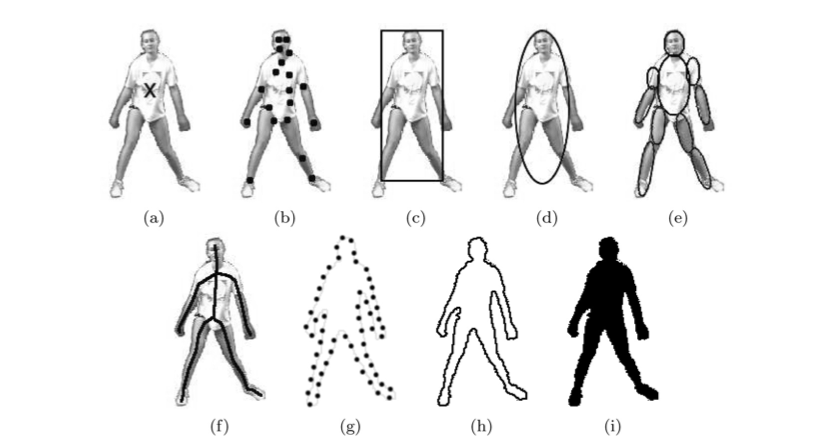
\includegraphics[scale=0.5]{figuras/2.FundamentacaoTeorica/representacao.png}
		\end{center}
		\caption{Representações de objetos rastreados. (a) Centróide, (b) múltiplos pontos, (c) representação retangular, (d) representação elíptica, (e) representação de múltiplas partes, (f) esqueleto do objeto, , (g) conotorno completo do objeto, (h) contorno do objeto por pontos, (i) silhueta do objeto~\cite{yilmaz}}
		\label{representacao}
	\end{figure}

	\begin{itemize}
		\item \textbf{Pontos:} o objeto é representado por um ponto, como por exemplo a centróide da Figura \ref{representacao}(a), ou por vários pontos, como por exemplo na Figura \ref{representacao}(b). Essa representaçao é mais adequada para rastreamento de objetos que ocupam uma pequena região na imagem;
		\item \textbf{Formas geométricas primitivas:} o objeto é representado por formas geométricas simples como um retângulo e uma elipse, como mostrados nas Figuras \ref{representacao}(c) e (d). Essa representação é mais adequada para simples objetos rígidos;
		\item \textbf{Silhueta e Contorno:} representação por contorno define os limites de um objeto, como mostrado nas Figura \ref{representacao}(g) e (h). A região interna do contorno é chamada de Silhueta, como mostrado na Figura \ref{representacao}(i). Essa represetação é mais adequada para rastrear objetos complexos de forma não rígida;
		\item \textbf{Modelos de formas articuladas:} objetos articulados são compostos por partes do corpo que se ligam por meio de juntas. Para representar objetos articulados, utiliza-se figuras geométricas para cada parte do corpo, como mostrado na Figura \ref{representacao}(e);
		\item \textbf{Modelos de Esqueletos:} modelos de esqueletos são extraídos do objeto rastreado, como mostrado na Figura \ref{representacao}(f). Essa representação pode ser utilizada tanto para objetos articulados rígidos quanto não rígidos;
	\end{itemize}

	Para rastreamento de pessoas a representação por meio de contorno ou silhuetas são as mais adequadas~\cite{yilmaz}.

%%%%%%%%%%%%%%%%%%%%%%%%%%%%%%%%%%%%%%%%%%%%%%%%%%%%%%%%%%%%%%%%%%%%%%%%%%%%%%%%%%%%%%%%%%%%%%%%%%%%%%%%%%%%%%%%%%%%%%%%%%%%%%%%%%%%%%%%%%%%%%%%%%%%%%%%%%%%%%%%%%%%%%%%%%%%%%%%%%%%%%%%%%%%%%%%%%%%%%%%%%%%%%%%%%%%%%%%%%%%%%%%%%%%%%%%%%%%%%%%%%%%%%%%%%%%%%%%%%%%%%%%%%%%%%%%%%%%%%%%%%%%%%%%%%%%%%%%%%%%%%%%%%%%%%%%%%%%%%%%%%%%%%%%%%%%%%%%%%%%%%%%%%%%%%%%%%%%%%%%%%%%%%%%%%%%%%%%%%%%%%%%%%%%%%%%%%%%%%%%%%%%%%%%

\subsection{Características para rastreamento}

	A seleção das características é uma tarefa crítica para o rastreamento e está fortemente relacionada com a representação do objeto. Em geral, a seleção procura as características mais singulares para que o objeto rastreado seja facilmente distinguido. As características mais comuns utilizadas autlamente são~\cite{yilmaz}:

	\begin{itemize}
		\item \textbf{Cor:} a cor do objeto é influênciada principalmente por duas características: a distribuição da iluminação e a propriedade de reflectância do objeto. Geralmente, o \textit{RGB} geralmente é utilizado para representar a cor;

		\item \textbf{Borda:} Os limites de um objeto gera uma grande variação na intensidade da imagem. A detecção por meio das bordas é utilizadado para identificar essas variações. As bordas são menos sensíveis a variações na iluminação comparado com as cores. Os algoritmos que detectam as bordas do objeto geralmente as utiliza para representação do mesmo;

		\item \textbf{Fluxo Óptico:} é um campo denso de vetores de deslocamento que define a tradução de cada pixel em uma região. Ele é calculado a partir da restrição de luminosidade, que pressupõe a constância de brilho de pixels correspondentes nas \textit{frames} consecutivas;

		\item \textbf{Textura:} é a medida da intensidade da variação da superfície que quantifica propriedades como suavidade e regularidade. A Textura é menos sensível a variação da iluminação comaprado com a cor;

	\end{itemize}
















% Adaptive Particle Filter with Body Part Segmentation for Full Body Tracking
% 	The existing full body tracking algorithms can be classified into two types. One is the method with monocular or multi-view images [2, 3, 4, 5], and the other is the method with 3D reconstructed data [1, 6, 7, 8]. The approaches with 2D images have the advantage that they work with a simple hardware setup. However, self-occlusion makes the 2D tracking problem hard for arbitrary movements. Thus the existing systems assume some a-priori knowledge of the type of movement and/or the viewpoint under which it is observed [9]. With the 3D reconstructed data we can process more kinds of action and


% Tracking Human Motion in Structured Environments Using a Distributed-Camera System
% 	2	SINGLE VIEW TRACKING
% 	Tracking from a single view includes two major components: preprocessing and feature correspondence between consecutive frames. Three stages of preprocessing are performed:
% 	Segmenting the moving objects from the still background, 
% 	Distinguishing human subjects from other segmented nonbackground objects, and Extracting features from the segmented human subjects.